\documentclass[a4paper,10pt]{article}
\usepackage[top=3cm, bottom=3cm, left=3cm, right=3cm]{geometry}

\usepackage[french]{babel}
\usepackage[utf8]{inputenc}
\usepackage[T1]{fontenc}

\usepackage[a4paper,colorlinks,linkcolor=darkgray,citecolor=red,urlcolor=blue]{hyperref}
\usepackage{pdfpages}
\usepackage{graphicx}
\usepackage{caption}
\usepackage{amsthm}
\usepackage{listings}


%% Trucs à marquer :
% extension des fichiers : .tricot
% contraintes à respecter (spilts, links, nbr maille multiple du nbr maille du motif), pour le nb de maille : conseil et le compil renvoie warning qd c'est pas le cas (et ne garantit pas de faire un truc cool) ?
%

%opening
\title{Documentation de TriLang}
\author{Équipe TriComp}

\begin{document}

\maketitle

\begin{abstract}

\end{abstract}

\newpage

\tableofcontents

\newpage


\section{Introduction}

\section{Description}

La description des ouvrages de tricot est basé sur le découpage en trapèzes : en effet, toute pièce tricotable est décomposable en un agencement de trapèzes
de dimensions variable.

En pratique, on décrit les pièces en donnant leurs dimensions (longueur des bases, hauteur) et le motif avec lequel elles seront remplies (jersey, point mousse,
côtes...).
% Ici : 

\section{Syntaxe}

  \subsection{Décrire vos points}

%% TO DO  
% Ici : où on décrit les points, et comment.
% Où : dans le fichier .tricot ? Ce serait le mieux mais est-ce que c'est possible facilement ?
% Comment : à décrire (type pattern = (int*((int* Maille of maille) list)) list où type maille = Endroit | Envers with sexp, compare)  

Il n'est pour l'instant pas possible de définir des points personnalisés, les points apparaissant dans les tricots doivent être choisis parmis les points suivants :
\begin{itemize}
\item jersey
\item point mousse
\item côtes 1/1
\item point de riz
\item côtes 2/2
\item fausses côtes anglaises
\item jersey rayé
\item côtes plates
\item côtes piquées
\item losanges
\item côtes point de riz
\item damier $3\times 3$
\end{itemize}
  
  \subsection{Commencer votre tricot}
  
Tout tricot commence par son son nom et sa description, donnés avec la syntaxe suivante :

%\begin{lstlisting}
\noindent \texttt{Name : [inserer ici le nom de votre ouvrage] \\
  Description : [inserer ici une description de votre ouvrage]} \\
%\end{lstlisting}

La description du tricot se fait ensuite en listant les pièces qui le compose. Une pièce est décrite avec la syntaxe suivante :

\noindent \texttt{piece [inserer ici le nom de votre pièce] := \\
  \textcolor{white}{alinea}start [insérer ici la largeur de votre pièce] \\
  \textcolor{white}{alinea}|| [insérer ici une description de votre pièce]}
  
La largeur de la pièce est donnée en nombre de maille et de manière générale, tous les entiers décrivant des tailles dans le langage sont donnés en nombre de mailles ou en nombre de rangs.

  \subsection{Décrire vos pièces}
  
  Les pièces sont composées de trapèzes qui sont assemblés grâce à des connecteurs.

\subsubsection{Un trapèze}

  La description d'un trapèze, unité atomique du tricot, se fait avec la syntaxe suivante : \\
\texttt{trapezoid (height : k, shift : $\mathtt{d_g}$, upper\_width : m, pattern : motif} où 
\begin{itemize}
\item \texttt{k} est la hauteur en rangs du trapèze
\item $\mathtt{d_g}$ est la différence (en mailles) entre la largeur du trapèze en haut et en bas
\item \texttt{m} est la largeur du trapèze en haut (la largeur en bas étant normalement inférable avec le reste du code
\item \texttt{motif} est simplement le point utilisé sur ce trapèze, à choisir parmi ceux listés plus haut
\end{itemize}

La figure \ref{trapeze} montre graphiquement ces paramètres sur un dessin.

\begin{figure}[!ht]
  \centering 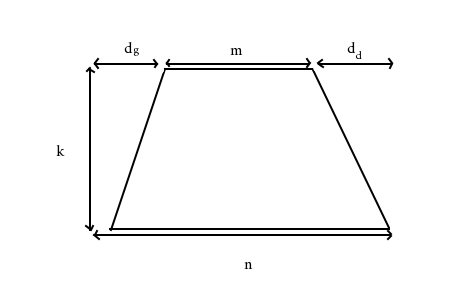
\includegraphics[scale=0.6]{../img/trapeze.jpg}
  \caption{Les paramètres d'un trapèze que l'on utilise}
  \label{trapeze}
\end{figure}

\subsubsection{Les connecteurs}

  
%%%%% %%%%%%%%%%%% ANNEXES %%%%%%%%%%%%%%%%%

\appendix

\section{Exemples}

Dans cette section, nous donnons des exemples complets de quelques modèles écrits grace à TriLang, allant du plus basique (écharpe) à des modèles plus compliqués (poncho et salopette). Un patron de ces modèles est également présenté, afin de rendre plus visuel ce que donne ces descriptions. Ces patrons ont été créés par l'interface graphique du logiciel TriComp.
% + exemples de définitions de points ?

\subsection{Écharpe}



\begin{lstlisting}
Name : scarf_test
Description : "The easiest knit you can make"

piece my_piece := start 25
   || trapezoid ( height : 150, shift : 0, upper_width : 25, pattern : jersey )
   || stop
\end{lstlisting}


\subsection{Poncho}

\begin{lstlisting}
Name : poncho_test
Description : "The poncho given in the midterm"


piece my_piece := start 60
   || trapezoid ( height : 100, shift : 0, upper_width : 60, pattern : garter )
   || split 0 30 { 
     trapezoid ( height : 30, shift : 0, upper_width : 15, pattern : envers )
     || trapezoid ( height : 30, shift : 0, upper_width : 30, pattern : envers )
     || link next 0
   }
   30 30 { 
     trapezoid ( height : 30, shift : 15, upper_width : 15, pattern : envers )
     || trapezoid ( height : 30, shift : -15, upper_width : 30, pattern : envers )
     || link next 30
   }


piece next := start 60
   || trapezoid ( height : 100, shift : 0, upper_width : 60, pattern : envers )
   || stop
\end{lstlisting}

\subsection{Salopette}

%\lstinputlisting{salopette.tricot}

\begin{lstlisting}
Name : salopette_test
Description : "Essai de description de la salopette decrite en reunion : 
version avec splits et links n-aires"

piece my_piece := start 50
   || trapezoid ( height : 200, shift : 0, upper_width : 50, pattern : envers )
   || link devant 0

piece jambe_2 := start 50
   || trapezoid ( height : 200, shift : 0, upper_width : 50, pattern : envers )
   || link devant 50

piece devant := start 100
   || trapezoid ( height : 100, shift : 0, upper_width : 100, pattern : envers )
   || split
   15 10 { trapezoid ( height : 30, shift : 0, upper_width : 10, pattern : envers )
     || link derriere 15 }
   75 10 { 
     trapezoid ( height : 30, shift : 0, upper_width : 10, lower_width : 10, 
       pattern : envers )
     || link derriere 75 }

piece derriere := start 10
   || trapezoid ( height : 100, shift : 0, upper_width : 100, lower_width : 100, 
     pattern : envers )
   || split
   0  50 { trapezoid ( height : 200, shift : 0, upper_width : 50, pattern : envers )
     || stop }
   50 50 { trapezoid ( height : 200, shift : 0, upper_width : 50, pattern : envers )
     || stop }
\end{lstlisting}

\end{document}
